\chapter{Ergebnisse}

= LÄNGSTES/AUSFÜHRLICHSTES KAPITEL!!!

Für jedes Unterkapitel gilt: 
> Erst allgemeines Vorgehen/Methodik definieren
> Danach spezifisch für jeden Browser: Unterschied zwischen Snapshot-Zeitpunkten, insb. zwischen Live- und Dead-Forensik

\section{Firefox}

\subsection*{White-Box Analyse/Common Locations}

Schreiboperationen mit Process Monitor verfolgen:

Allgemein: Nur Dateien untersucht, die gemäß Methodik (Kapitel X) entweder im Snapshot vorhanden sind oder sich über Autopsy Carving PlugIn bzw. RAM wiederherstellen lassen.
> Wenn Temp-Dateien nicht mehr vorhanden, wird die nicht-Temp Datei aufgeführt
> SQLite: um DBs auswerten zu können, werden alle WAL-Dateien mittels PRAGMA Checkpoint in die .sqlite-Datei überführt

Ergebnis: Tabelle mit wiederherstellbaren Dateien: Logfile 1 vs. Logfile 2 + Tool mit dem Datei untersucht wurde
\begin{figure}[h!]
	\resizebox{\linewidth}{!}{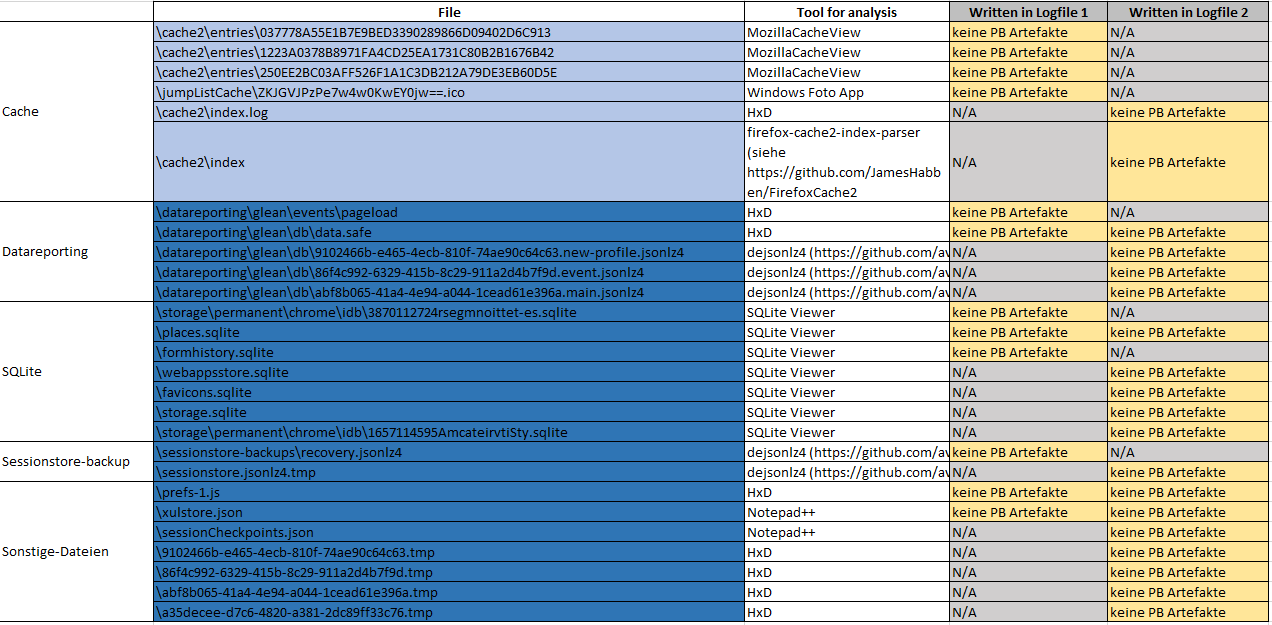
\includegraphics{bilder/firefox-tabelle-logfile1vlogfile2-reduced.png}}
%	\label{...}
	\caption{Tabelle mit wiederherstellbaren Dateien: Logfile 1 vs. Logfile 2}
\end{figure}

Im Anhang: Tabelle mit allen geschriebenen Dateien (markiert, wenn nicht mehr wiederherstellbar + markiert, wenn Datei "verändert" (siehe oben: temp, WAL))

Kategorien der Logs:
- Common Paths:
	(Local) %C:\Users\Forensik\AppData\Local\Mozilla\Firefox\Profiles\<Profile>.default-release\
	(Roaming) %C:\Users\Forensik\AppData\Roaming\Mozilla\Firefox\Profiles\<Profile>.default-release\

> TODO: Bei diesen Dateien gleich Diff beschreiben => SQLite-Dateien gesondert betrachtet
- Cache: 
	Logfile 1:
		> % \cache2\entries\037778A55E1B7E9BED3390289866D09402D6C913 (Local)
		> % \cache2\entries\1223A0378B8971FA4CD25EA1731C80B2B1676B42 (Local)
		> % \cache2\entries\250EE2BC03AFF526F1A1C3DB212A79DE3EB60D5E (Local)
		> % \jumpListCache\ZKJGVJPzPe7w4w0KwEY0jw==.ico (Local)
			Enthält kleines "m" Icon
	Logfile 2:
		> % \cache2\index (Local)
		> % \cache2\index.log (Local)
			=> Untersucht mit HxD
- datareporting:
	=> dekomprimiert mit dejsonlz4
	Logfile 1:
		> % \datareporting\glean\events\pageload (Roaming)
		> % \datareporting\glean\db\data.safe (Roaming)	
	Logfile 2:
		*> % \datareporting\glean\db\data.safe (Roaming)
		> %  \datareporting\glean\db\9102466b-e465-4ecb-810f-74ae90c64c63.new-profile.jsonlz4 (Roaming)
		> % \datareporting\glean\db\86f4c992-6329-415b-8c29-911a2d4b7f9d.event.jsonlz4 (Roaming)
		> % \datareporting\glean\db\abf8b065-41a4-4e94-a044-1cead61e396a.main.jsonlz4 (Roaming)
			enthält Systeminformationen
- Sessionstore-Backup:
	=> dekomprimiert mit dejsonlz4
	Logfile 1:
		> % \sessionstore-backups\recovery.jsonlz4 (Roaming)
			mit Tool: Tab 1:  Willkommen bei Firefox [6.5.2023, 22:25:06, about:welcome;
			Tab 2:  Firefox Datenschutzhinweis — Mozilla [6.5.2023, 22:24:59], % https://www.mozilla.org/de/privacy/firefox/
			(Gleicher Inhalt in recovery.baklz4)
	Logfile 2:
		> % \sessionstore.jsonlz4
			nein, nach Dekompression image-Eintrag als base64 entdeckt: "m" Icon
			(https://base64.guru/converter/decode/image)
- Sonstige Dateien:
	Logfile 1:
		> % \prefs-1.js
		> % \xulstore.json			
	Logfile 2:
		*> % \prefs-1.js (Roaming)
		*> % \xulstore.json (Roaming)
			neuer Eintrag "sidebar-box"
		> % \sessionCheckpoints.json (Roaming)
		> % \9102466b-e465-4ecb-810f-74ae90c64c63.tmp (Roaming)
		> % \86f4c992-6329-415b-8c29-911a2d4b7f9d.tmp (Roaming)
		> % \abf8b065-41a4-4e94-a044-1cead61e396a.tmp (Roaming)
		> % \a35decee-d7c6-4820-a381-2dc89ff33c76.tmp (Roaming)
- SQLite: (TODO: Abgleich mit Diffs-Exceltabelle, ob wirklich nur in places.sqlite geschrieben wurde)
	=> Untersucht mit SQLite-viewer
	=> Diff mit sqldiff
	=> Checkpoints mit PRAGMA wal\_checkpoints
	=> SQLite Diff Tabelle 
	Logfile 1:
		> % \storage\permanent\chrome\idb\3870112724rsegmnoittet-es.sqlite (Roaming)
		*> % \places.sqlite (Roaming)
		> % \formhistory.sqlite (Roaming)
	Logfile 2:
		*> % \places.sqlite (Roaming)
		> % \formhistory.sqlite (Roaming)
			This file remembers what you have searched for in the Firefox search bar and what information you’ve entered into forms on websites.
			% (https://support.mozilla.org/en-US/kb/profiles-where-firefox-stores-user-data)
		> % \webappsstore.sqlite (Roaming)
		> % \favicons.sqlite-wal (Roaming)
		> % \storage.sqlite (Roaming)
		> % \storage\permanent\chrome\idb\1657114595AmcateirvtiSty.sqlite (Roaming)
			> IndexedDB-Dateien, sind DBs, die von besuchten Webseiten
			angelegt werden % (https://www.reddit.com/r/firefox/comments/dri650/what_are_the_idb_files_in_the_permanent_storage/)
			> Im Chrome-Ordner: "the databases in the chrome subfolder relate to various pieces of integrated firefox functionality (content for the new tab page, blocklists, shield/normandy, remote settings, push api, ...)"
			> Enthalten eigentlich URL im Dateinamen
			> TODO: können geparsed werden: % https://stackoverflow.com/a/59923297/18037004
			"Activity Stream for Firefox is a collection of all the things you do in the browser that you care about displayed in a rich and meaningful way" 
			%https://wiki.mozilla.org/Firefox/Activity_Stream
			--> DB enthält keine Browsing Artefakte

Zusammenfassung:
	Allgemein: Nur 4 Schreiboperationen auf Dateien, die in 1. Logfile (mit * markiert) beschrieben wurden => TODO: für Sqlite Datien prüfen

Quantitativ: (Diagramme)		
	> Gestacktes Balkendiagramm zu veränderten SQLite DBs
	\begin{figure}[h!]
		\centerline{\resizebox{0.7\linewidth}{!}{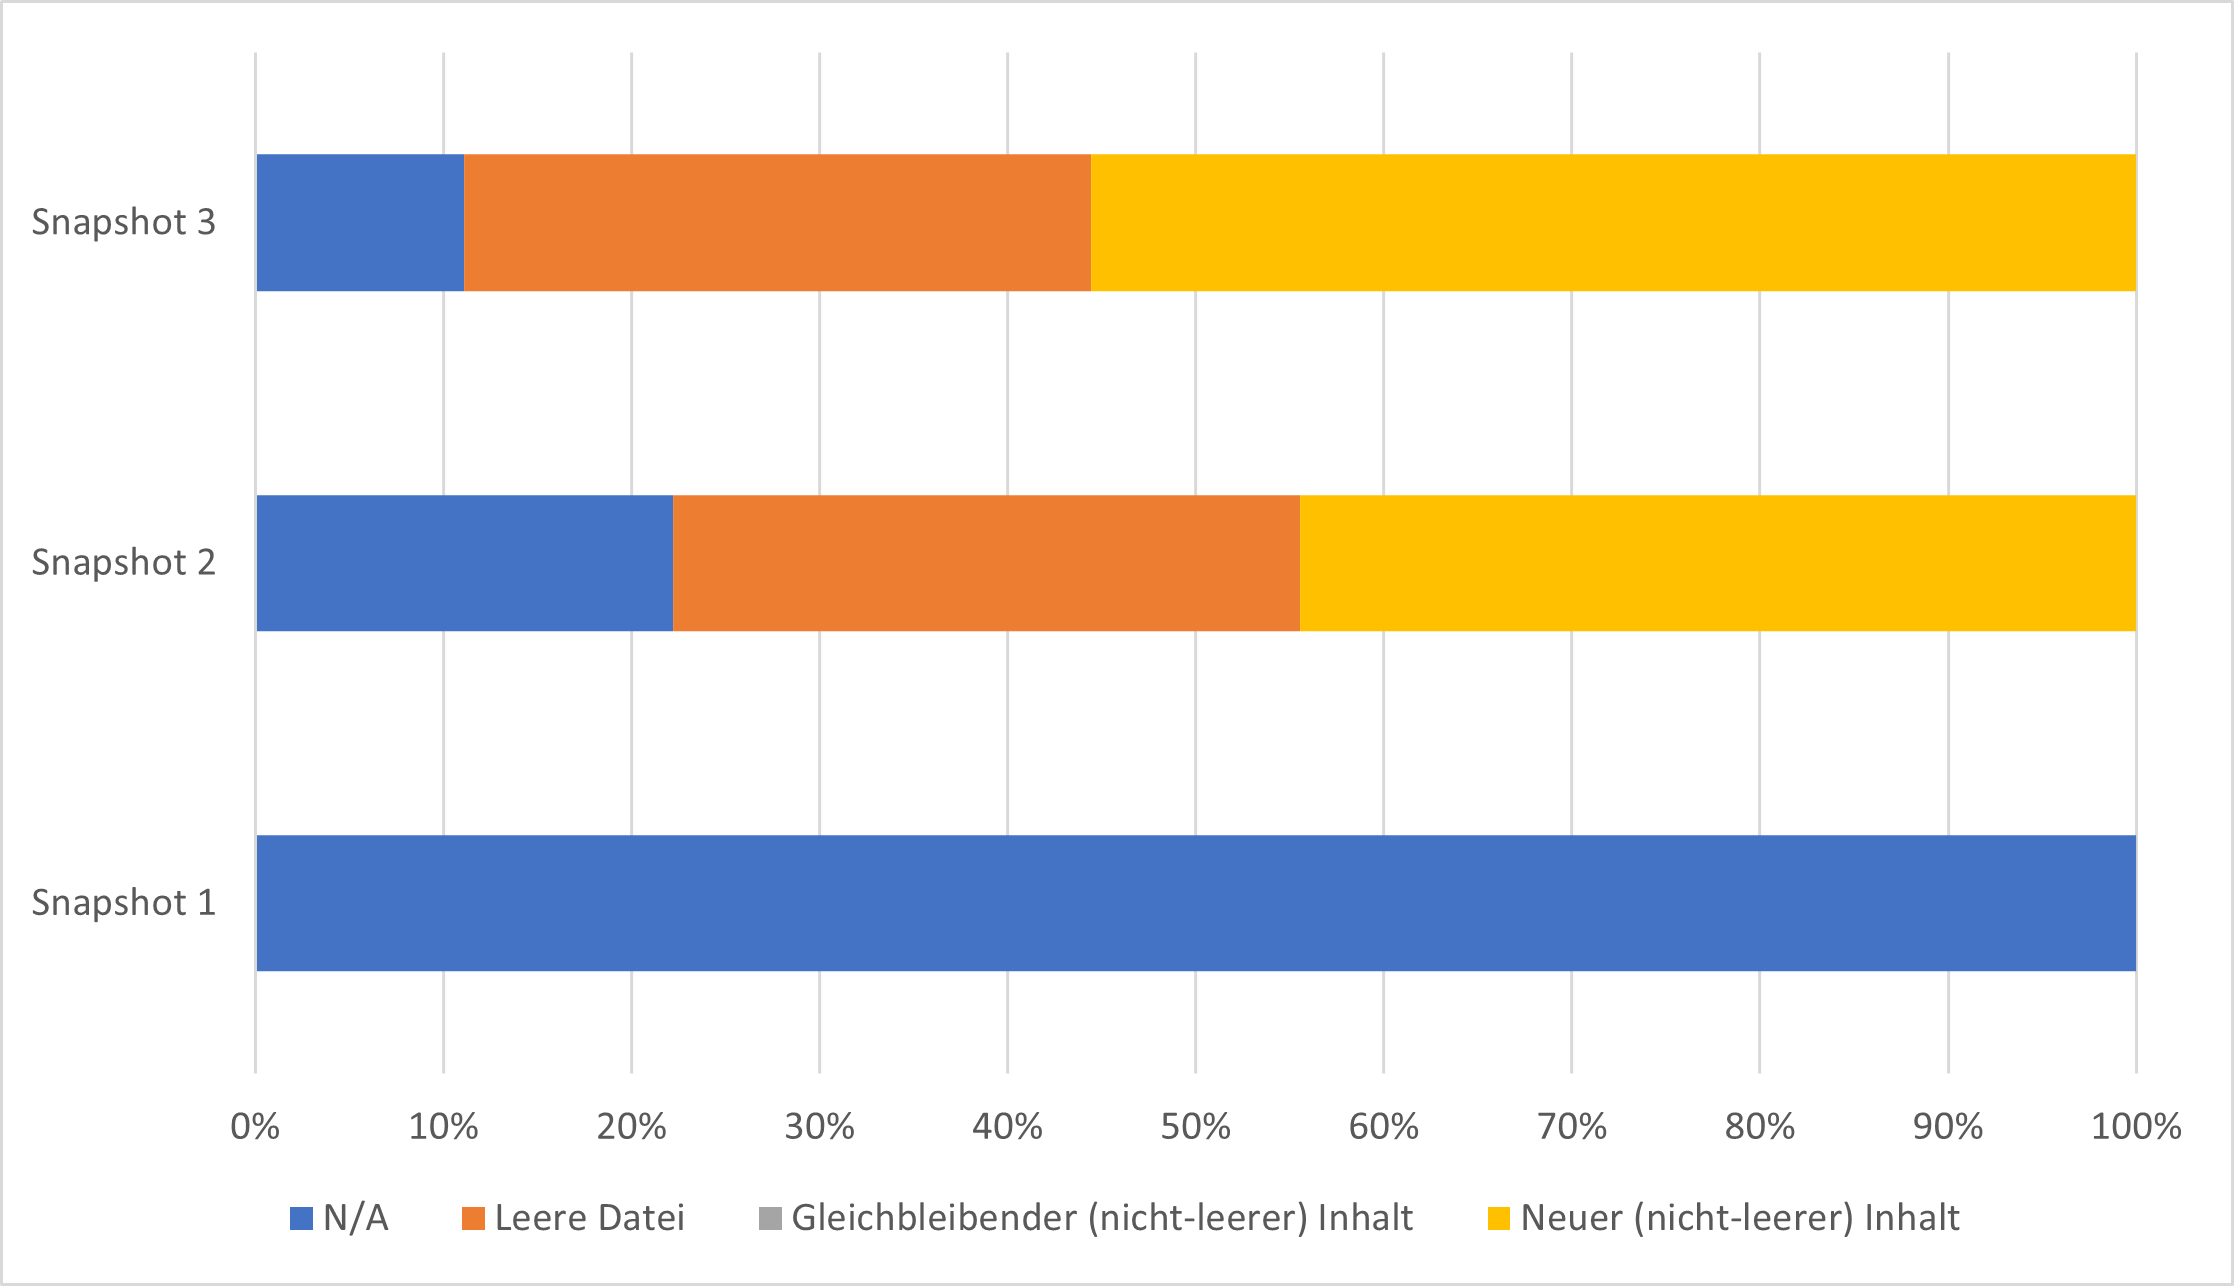
\includegraphics{bilder/firefox-stacked-bar-chart-sqlite-test.png}}}
		\label{chart:final-criteria}  
		\caption{Comparison of found PB artifacts between RAM Dumps}
	\end{figure}
	> Balkendiagramm: Für jede Logfilekategorie: Anzahl Schreiboperationen Logfile 1 vs Logfile 2
	\begin{figure}[h!]
		\centerline{\resizebox{\linewidth}{!}{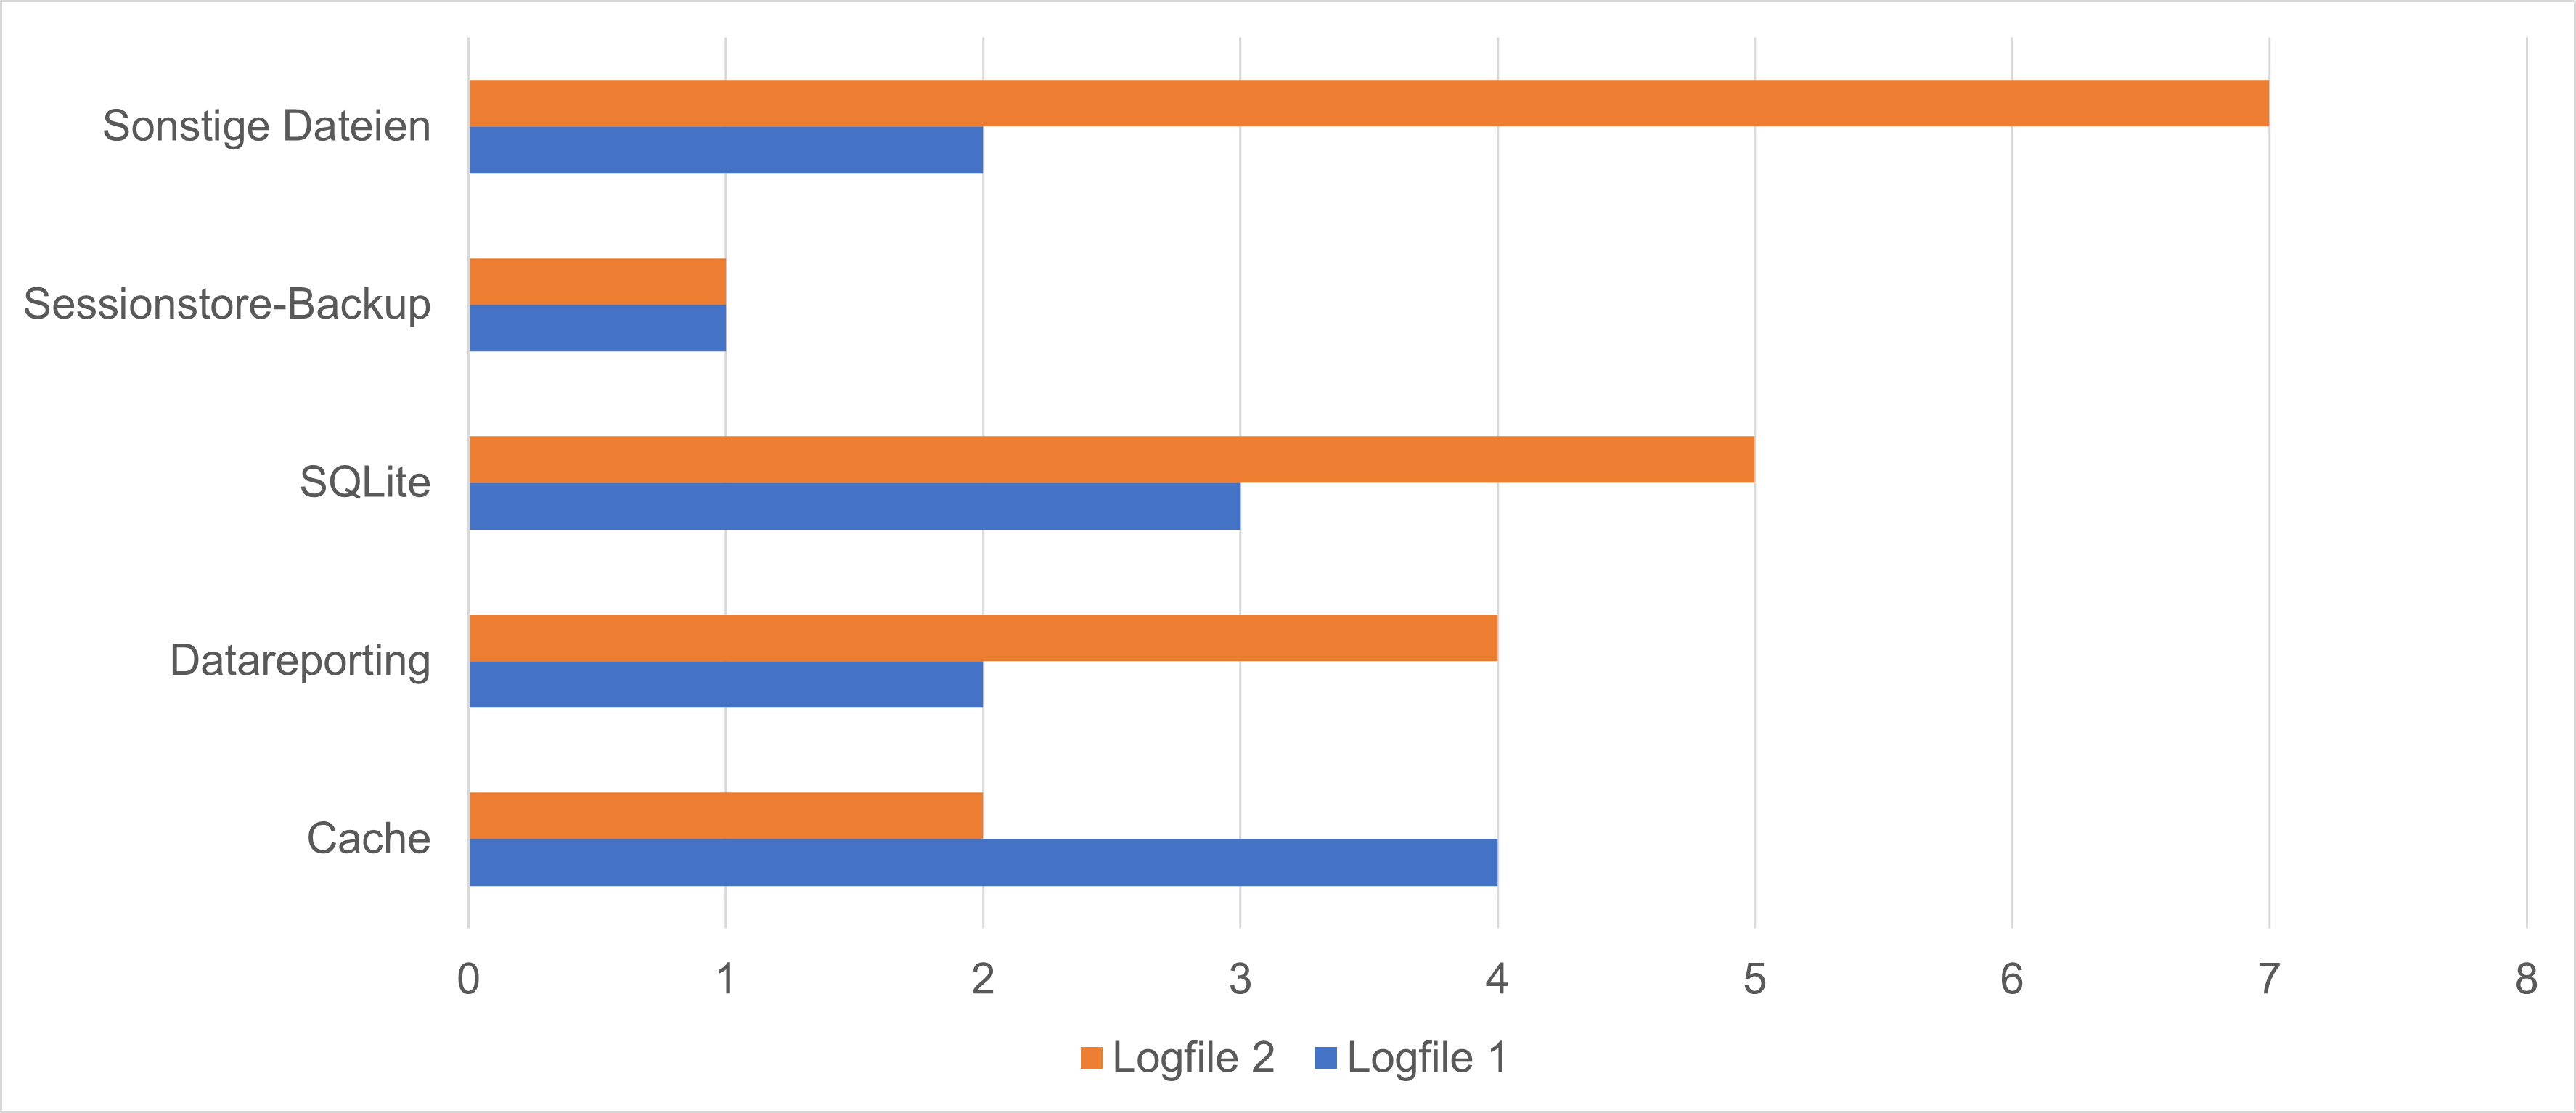
\includegraphics{bilder/bar-chart-logfile1vs2-test.png}}}
		\label{chart:final-criteria}  
		\caption{Comparison of found PB artifacts between RAM Dumps}
	\end{figure}

Literatur:
	o no traces were found in “common locations” \cite{Montasari.2015}
		>  “places.sqlite”, “webappsstore. sqlite”, “sessionstore.bak”, “search.json” and “nssckbi.dll”
	o	Safebrowsing: Alle Dateien in /safebrowsing-updating/ nicht relevant. Dort nur .vlpset und .sbstore Dateien. Speichern 256-Bit Hash von URLs, die auf SafeSearch Blacklist stehen 
	o	Cache-Dateien: drei Caches: startupCache, jumpListCache (beide enthalten Binärdateien ohne Browsing Artefakte) und cache2 (können mit MozillaCacheView untersucht werden, enthalten keine Browsing Artefakte)
	o	SQLite Datenbanken: Sqlite Dateien erst ohne WAL Dateien untersuchen, Danach mit sqlite3 Konsole: WAL in Datenbank schreiben mit: PRAGMA wal\_checkpoint; places.sqlite besonders relevant, da dort Browser in public Modus Browsing URLs verwaltet (Am besten hier vergleich mit Public Browsing machen)	
		> \cite{Fayyad.2021} for Mozilla Firefox, 7 database files were recovered: cookies.sqlite-shm, places.sqlite-shm, prefs.js etc.
		> \cite{Muir.2019} The two SQLite databases used by Firefox to track cookies and history (cookies.sqlite und places.sqlite) were both recoverable from the file system after deletion	
		Ergebnisse stehen im Gegensatz zu \cite{Hedberg.2013} :
			o	Chrome und Firefox: Einträge in places.sqlite + history.sqlite DB gefunden während PB! (Noch aktuell??)
		Sonderfall: SQlite DB-Crash \cite{Hedberg.2013}
			> WAL Files/Journal Files bei Crash gefunden -> Kann genutzt werden um zu beweisen, dass privater Browser genutzt wurde
			> Daher: WAL Rollback mit sqlite3	
	o	Jsonlz4 \& balkz4: Enthalten komprimierte Firefox-Sessions, jsonlz4 Dateien können mit Tool "entkomprimiert" werden: https://www.jeffersonscher.com/ffu/scrounger.html


\subsection*{Registry}
> Process Monitor: SetValue Operationen von Browser 
	Kategorien Registry Keys:
	1) PreXULSkeletonUISettings:
		> UI Einstellungen von Firefox (TODO: Quelle) 
		> Struktur der Keys: % HKCU\SOFTWARE\Mozilla\Firefox\PreXULSkeletonUISettings\C:\Program Files\Mozilla Firefox\firefox.exe|<UI Einstellung>
		> Unterschiedliche UI Einstellungen
			- % ScreenX (DWORD)
			- % ScreenY (DWORD)
			- % Width (DWORD)
			- % Height (DWORD)
			- % Maximized (DWORD)
			- % Flags (DWORD)
			- % CssToDevPixelScaling (REG_BINARY)
			- % UrlbarCSSSpan (REG_BINARY)
			- % SearchbarCSSSpan (REG_BINARY)
			- % SpringsCSSSpan (REG_BINARY)
		> keine PB Artefakte unter UI Einstellungen	
	2) Business Activity Monitoring % https://learn.microsoft.com/de-de/biztalk/core/business-activity-monitoring-bam
		> Quelle: % https://notes.qazeer.io/dfir/windows/_artefacts_overview
		> BAM is a mostly undocumented feature that controls the programs executed in the background. DAM is a feature for devices supporting the "Connected Standby" mode (i.e when a device is turned on, but its display will be turned off). As a result, the BAM registry keys will contain data on any devices, while DAM registry keys will only contain data on mobile devices.
		> The BAM registry key contains multiple subkeys under bam\\State\\UserSettings, with one subkey per user, identified with the user SID. While the key is in the SYSTEM registry hive, program executions can thus still be tied to a specific user using this SID.
		> Each user-specific key contains a list of executed programs, with their full path and timestamp of last execution.
		> If a file is deleted, the eventual associated entry in the BAM is deleted as well after the system reboot. Additionally, BAM entries older than 7 days are deleted upon system boot. The BAM thus provides limited information on historic execution of programs
		> No entries are created in the BAM keys for executables on removable media and/or on network shares.
		> Key: %  HKLM\System\CurrentControlSet\Services\bam\State\UserSettings\S-1-5-21-588412547-2749917301-3803556669-1001\\Device\HarddiskVolume2\Program Files\Mozilla Firefox\firefox.exe (REG_BINARY)

Quantitativ: (Diagramme)
	- Stacked Balkendiagramm jeweils für Logfile 1 und Logfile2: Anteil Kategorie 1 bzw.2 an allen Registry-Schreiboperationen

> Stringsuche in Registry Hives mit Registry Explorer (Siehe Liste)
	In allen Hives kein Treffer für alle Suchbegriffe

> "shellactivities-ähnliche" Keys untersucht
	TODO!
	
Literatur:
	>	Auf Autor verweisen: angeblich in Shellactivities Ergebnisse. --> Nicht mehr vorhanden in aktueller Version (Verweis auf E-Mail)
	>	Process Monitor/Regshot zeigen keine relevanten Key-Änderungen
	> \cite{Muir.2019}: Autopsy Keyword Suche nach Suchbegriffen: Ergebnisse in \%SystemRoot\%Minidump NTUSER.DAT, ntuser.dat.LOG1 (a log of changes to NTUSER.DAT)
	> Zentral: shellactivites Key:	NTUSER.DAT --> “shellactivities” key \cite{Muir.2019}
	> \cite{Rochmadi.2017} Detection of registry changes helps to determine what the appropriate plugin is used to search for digital evidence using volatility memory forensic:
	- RegQueryValue:	HKCU/Software/Microsoft/Windows/CurrentVersion/InternetSettings/Connections/DefaultConnectionSettings
	- RegCloseValue: 	HKCU/Software/Microsoft/Windows/CurrentVersion/InternetSettings/Connections
	- IRP\_MJ\_READ: C:/pagefile.sys


\subsection*{Black-Box Analyse/Uncommon Locations}

\subsubsection*{Analyse mit Autopsy}
Bei White-Box Analyse: Autopsy nur zur Dateiextraktion genutzt, hier: als konkretes forensisches Werkzeug

Qualitative Analyse:

Stichwortsuche:
- In allen Snapshots keine Treffer (auch innerhalb \$Carved)
- TODO: Pagefile gefunden?

Plug-Ins:
- Web Bookmarks:
	Snapshot 2:
		> 5 Einträge in places.sqlite: (Firefox Standardseiten -> Deckt sich mit Beobachtungen aus Process Monitor Analyse)
		> Bing.url (Unter C:/User/Forensik/Favorites/Links) enthält Bing Startseite
- Web Cookies:
	Snapshot 2:
		> 10 Einträge in WebCacheV01.dat (= DB des Internet Explorers zum speichern von Browserdaten): Cookies für bing.com und live.com (= outlook)
- Web History:
	Snapshot 2:
		> 1 Eintrag in places.sqlite: % https://www.mozilla.org/privacy/firefox/
			-> Zurückzuführen auf Seite, die sich automatisch geöffnet hat, als Firefox gestartet (bevor privates Fenster geöffnet wurde)
		> 3 Einträge in WebCacheV01.dat:
			- 2x live.com (= outlook)
			- file:///Z:/Logfile\_1 (= Process Monitor Logfile, die in shared-Folder geladen wurde) -> Erklärung?
- Web Categories:
	Snapshot 2:
		> 2x WebCacheV01.dat aufgelistet => Mit HxD untersucht, keine PB Artefakte

Literatur:
	o	Autopsy Keywortsuche: 
		>	In alles Snapshots ergebnislos (keine Keyword-Hits
		-->	In Literatur: Autoren fanden Ergebnisse in pagefile.sys 
			> Autopsy: websites and some of the keywords found in hidden file called “pagefile.sys” \cite{Mahlous.2020}
			o \cite{Montasari.2015} traces were found in: 
				> However, on investigating the “pagefile.sys”, some entries were discovered
				> Using the “data carving” technique, profile picture was recovered
			o \cite{Said.2011} 
				> Examining pagefile.sys showed some positive hits 			
		--> Evtl. hier zeigen, was gefunden werden kann, wenn RAM reduziert
		--> Aber auf Problem hinweisen, dass gefundener String in pagefile nicht direkt Browser zugeordnet werden kann
		> \cite{Gabet.2018}	Firefox only produced three recoverable artefacts as reported by both tools (FTK, Autopsy) --> Artefakte werden nicht genannt!
		> \cite{Muir.2019} Autopsy Keyword Suche nach Suchbegriffen: unallocated space
		> Autopsy Carving Module (\$Carved): \cite{Muir.2019}
			•	When searching for the string ’clot’ from the browsing protocol, six .dll, .edb and .reg files were discovered in unallocated space.
			•	Further searching of unallocated space uncovered references to the Tor installation directory and the obfs4 bridging IP addresses
			•	browsing data found in NTUSER.DAT was also replicated in unallocated space.
	o	Autopsy PlugIns:
		>	*** TODO: Hier Liste mit PlugIns ***

\subsubsection*{Analyse mit Volatility}
Vorgehen: Siehe "Methodik" Kapitel
	- Ausgangslage: Volatility Yarascan Treffer
	- Für jeden Treffer: virtueller Offset des Strings, PID, getriggerte Yararule, getriggerte Yara Component z(= Variablenname des gesuchten Strings), gefundener String
	- Neue Spalte: "Prozessname" -> zu jeder PID Prozessnamen
	- Ergebnisse Aufbereitet nach folgendem Schema:
		> Für jeden RAM Dump
		> Für jede Yararule
		> Für jede Component
		> Filter: Prozessname = Firefox -> Anzahl zählen
		> Filter: Prozessname = Alle Prozesse außer Firefox -> Anzahl zählen

Quantitative Auswertung:
	- RAM Dump 1: 0 Yarascan-Treffer
	- RAM Dump 2: (Nach Browsing Szenario, Browser noch geöffnet)
		\captionsetup[subfigure]{labelformat=empty}
		\begin{figure}[h!]
			\small
			\centering	
			\subfloat[]{
				\resizebox{!}{5cm}{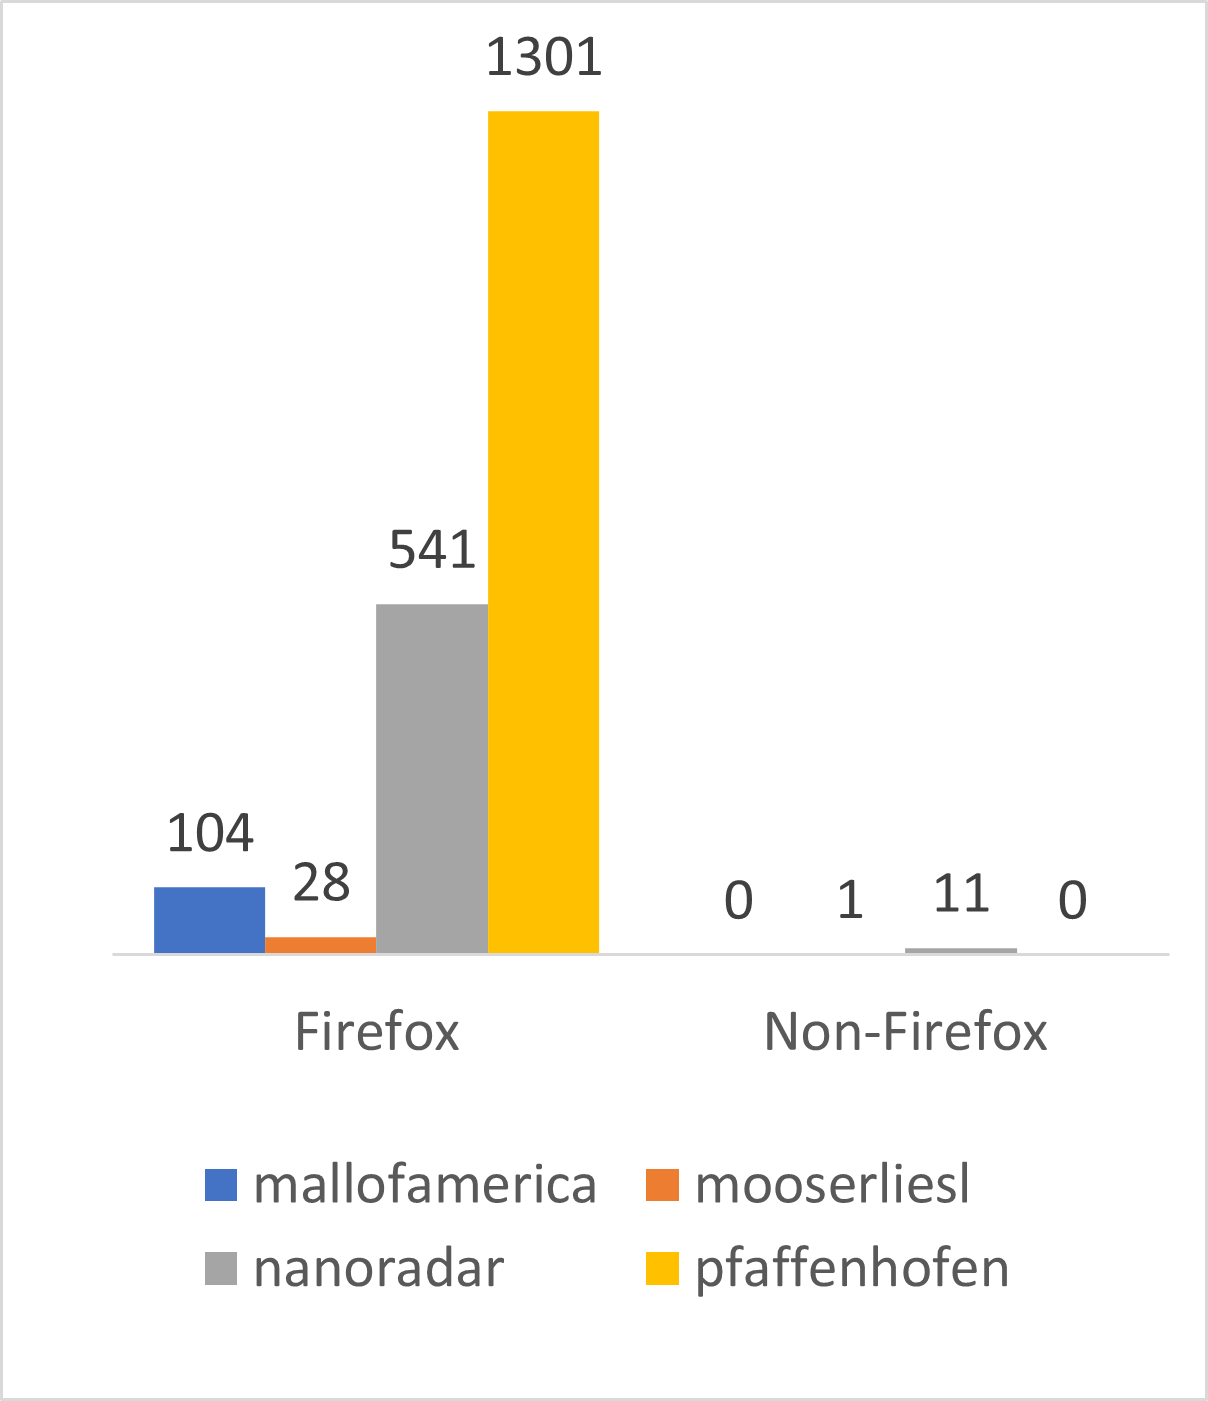
\includegraphics{bilder/bar-chart-test-1.png}}
			}
			\hspace*{\fill}
			\subfloat[]{           
				\resizebox{!}{5cm}{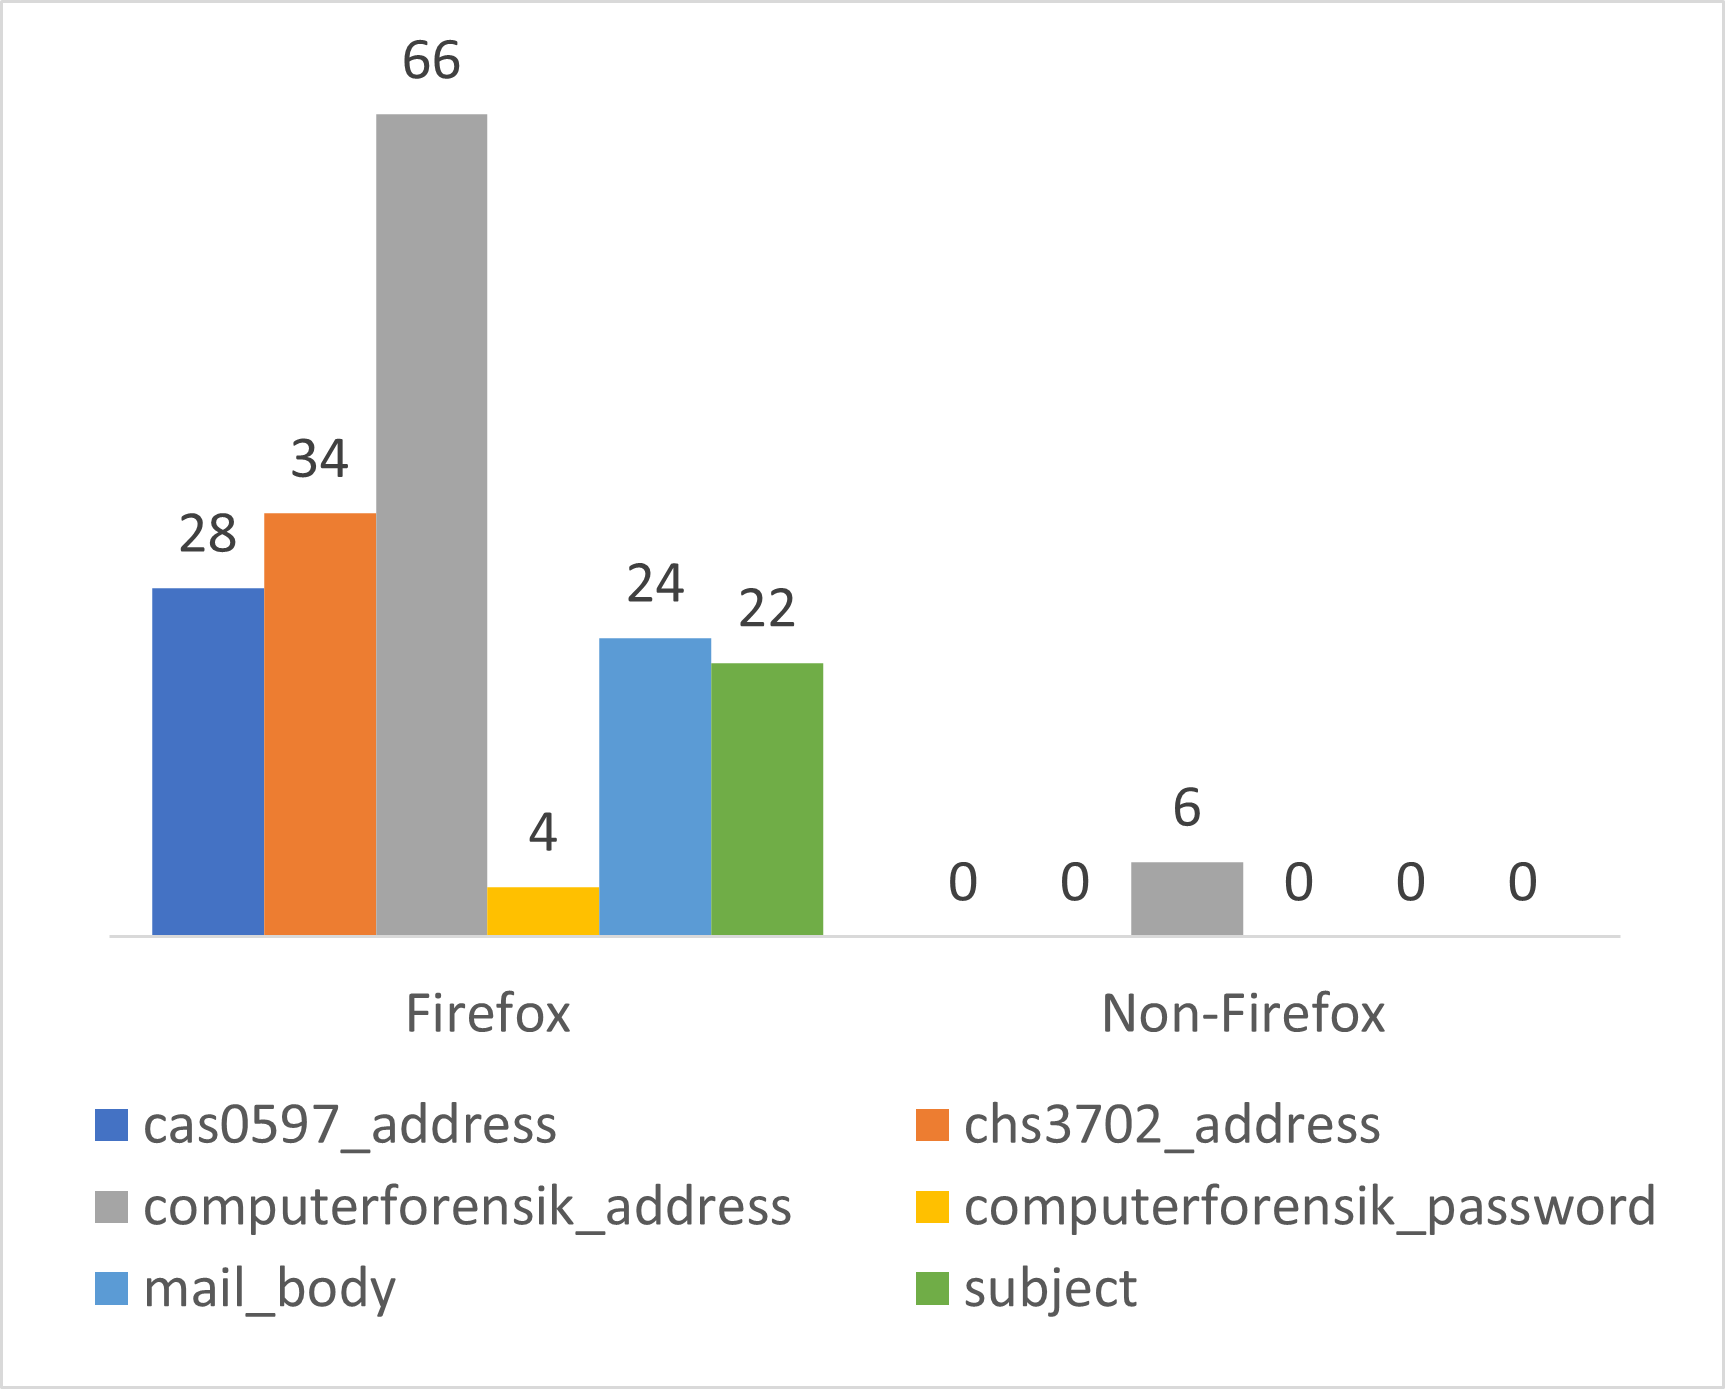
\includegraphics{bilder/bar-chart-test-2.png}}
			}
			\hspace*{\fill}
			\subfloat[]{           
				\resizebox{!}{5cm}{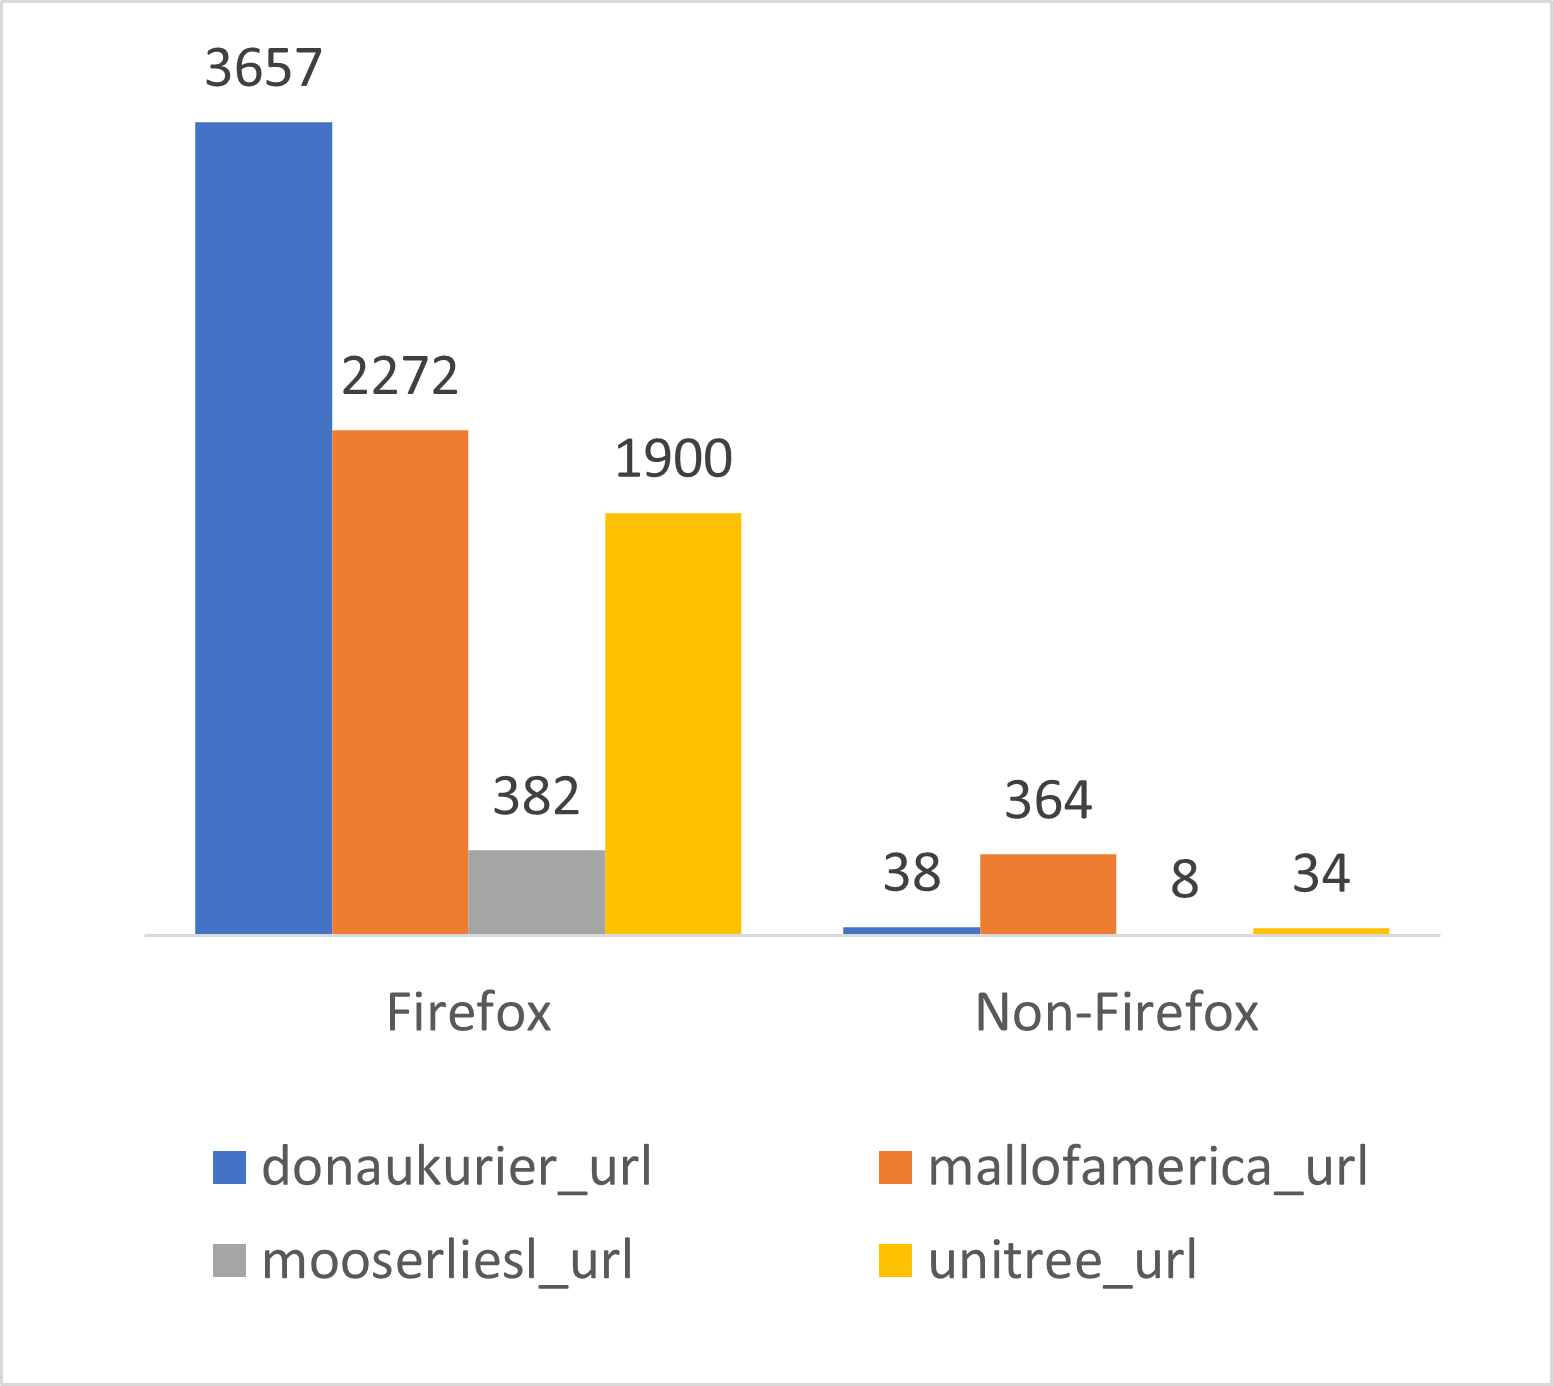
\includegraphics{bilder/bar-chart-test-3.png}}
			}
			\label{chart:final-criteria}  
			\caption{PB Artifacts found in RAM Dump 1}
		\end{figure}	
		Yararule "Keyword":
			> Firefox: 1974x
			> Non-Firefox: 12x
		Yararule "URL"
			> Firefox: 8211x
			> Non-Firefox: 444x		
		Yararule "Mail":
			> Firefox: 1974x
				=> Absenderadresse so häufig wie Empfängeradressen zusammen
				=> PW im Klartext 4x!
			> Non-Firefox: 12x
		Yararule "Image":
			> TODO!
	- RAM Dump 3: (Nach Browsing Szenario, Browser geschlossen)
		TODO!

Zusammenfassung = Stacked Bar Chart:
\begin{figure}[h!]
	\resizebox{\linewidth}{!}{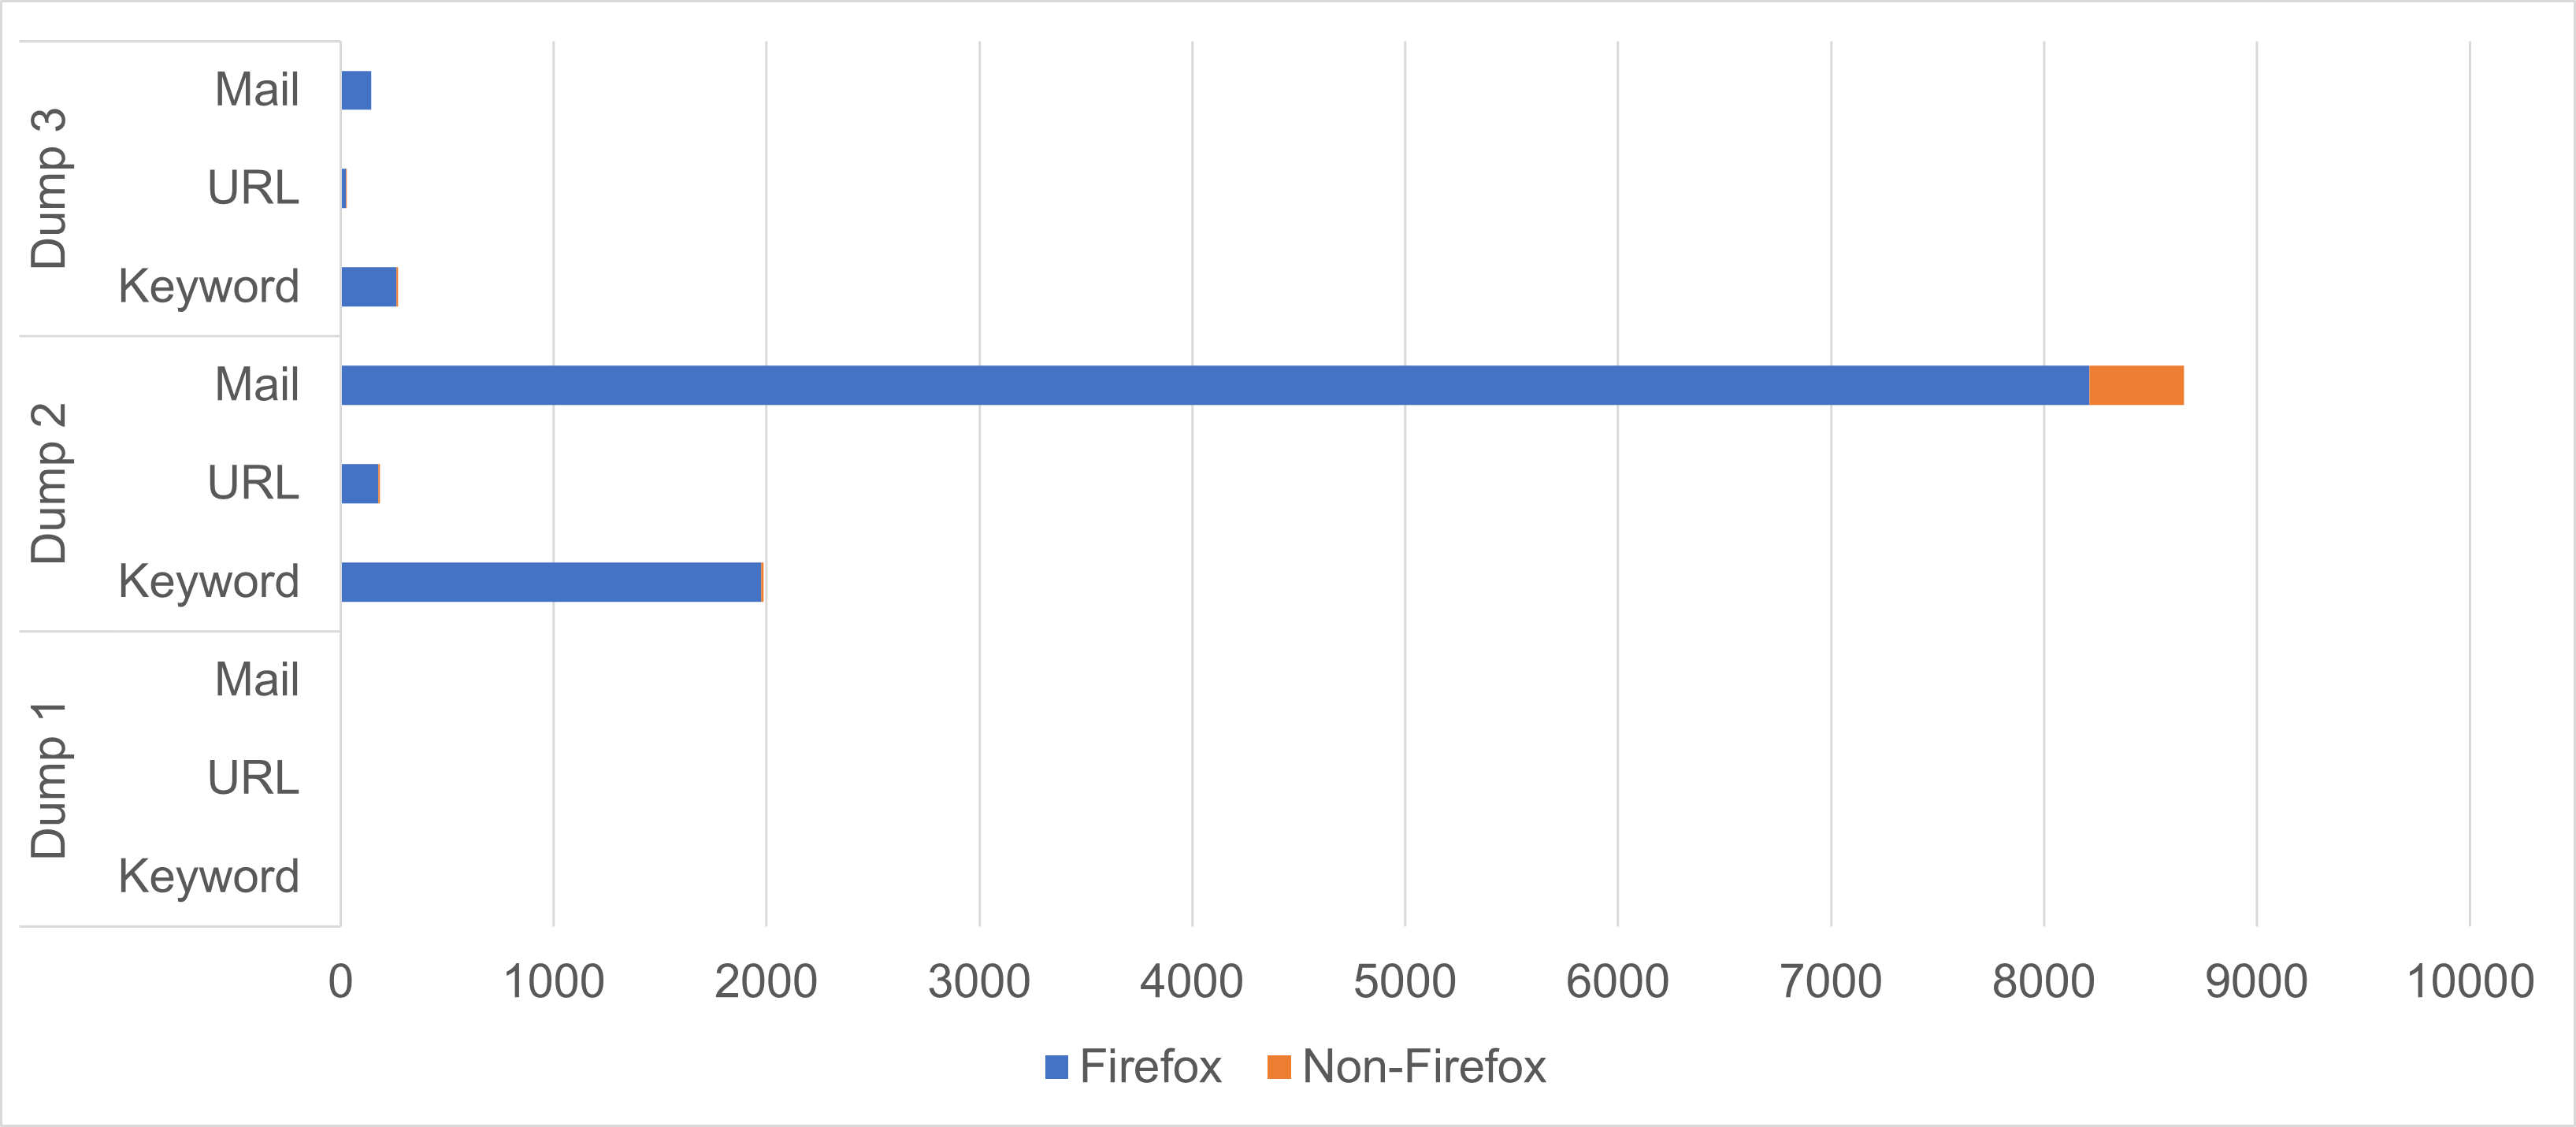
\includegraphics{bilder/stacked-bar-chart-test.png}}
	\label{chart:final-criteria}  
	\caption{Comparison of found PB artifacts between RAM Dumps}
\end{figure}

TODO: Kreisdiagramme/Balkendiagramme mit Gesamtzahl an (Non-)Firefox Yarascan-Treffer erst im Vergleich mit Tor

\section{Tor}

\subsection*{Uncommon Locations}

\subsubsection*{Qualitative Analyse}

o Autopsy: \cite{Muir.2019}
	•	Configuration files, downloaded files, and browserrelated data are recoverable from the file system.
	•	Significant data-leakage from the browsing session occurred: HTTP header information, titles of web pages and an instance of a URL were found in registry files, system files, and unallocated space.



o RAM-Analyse nach \cite{Muir.2019}:
	•	Live-Analyse identifiziert auch nach dem Schließen und Deinstallieren des Browsers und Abmelden des Benutzers Spuren von Tor-Prozessen, einschließlich des absoluten Pfads zur Browser-Executable, des Benutzernamens und des Geräts, von dem es ausgeführt wurde.
	•	The data-leakage contained the German word for ’search’ in reference to a Google search. This hints at the locale of the Tor server used to exit the network (exit relay).

o RAM-Analyse nach \cite{Hariharan.2022}:
	o	process was found to be firefox.exe
	o	pslist and pstree: parent process was shown 
	o	Belkasoft Ram Capturer: retrieve information about facebook
	o	Cmdline: file path of the browser “E:/TorBrowser/Browser/firefox.exe” + name of process tor.exe and firefox.exe
	o	Dlllist: DLL files of the executable files were not captured
	o	Netscan: tor.exe + obfs4proxy.exe -> showed “LISTENING” connections to nonstandardized ports as output.
	Yarascan: was able to retrieve all the browsing sessions
o RAM-Analyse nach \cite{Sajan.2021} mit Volatility
	•	process list extracted from the memory
	•	registry hives been extracted from the memory dump
	•	threads were extracted: “D:/VolatilityWorkbench/volatility.exe”–plugins=”D:/VolatilityWorkbench/profiles” pslistfilename =”C:/Users/username/Desktop/tor.raw” –profile=Win10x64 17763 –kdbg=0xf807606ac5e0
	•	Handles: resources used by the process 5672
	•	Dlls: These dlls can be found from prefetch file --> Can be found in “prefetch” file -> Analyzed with “winprefetchview”
	•	Places.sqlite: SQLite viewer has been used to recover bookmarks and frequently visited sites even after uninstalling the application
	•	Visited Websites: Using keyword search in Dump’s Hex

o Registry:
	> Shellactivites (siehe Firefox) \cite{Muir.2019}: instance of a URL were found in registry file
	> \cite{Nelson.2020} The userassist key is located in the NTUSER.dat hive of the
		 -> Registry and indicates the execution path of the program, as well as the number of times the program was executed 

\subsubsection*{Quantitative Zusammenfassung}



\section{Chrome}

\subsection*{Uncommon Locations}

o Autopsy Keyword-Suche: 
	> Chrome and Edge produced five artefacts as reported by both tools. (FTK, Autopsy) \cite{Gabet.2018}
		--> Artefakte werden nicht genannt!
	> only two temporary files (Figure 7) were recovered with Minitool Power Data Recovery but it was a dead end; Location: appdata/…/Chrome/…/ Preferences/RF1533fa.TMP \cite{Fayyad.2021}
	> pagefile.sys file showed no traces at all \cite{Said.2011}
	

\section{Brave}